% Created 2010-10-16 Sat 14:06
\documentclass[11pt]{article}
\usepackage[utf8]{inputenc}
\usepackage[T1]{fontenc}
\usepackage{fixltx2e}
\usepackage{graphicx}
\usepackage{longtable}
\usepackage{float}
\usepackage{wrapfig}
\usepackage{soul}
\usepackage{textcomp}
\usepackage{marvosym}
\usepackage{wasysym}
\usepackage{latexsym}
\usepackage{amssymb}
\usepackage{hyperref}
\tolerance=1000
\usepackage{color}
\usepackage{listings}
\lstset{
keywordstyle=\color{blue},
commentstyle=\color{red},
stringstyle=\color{green},
basicstyle=\ttfamily\small,
columns=fullflexible,
basewidth={0.5em,0.4em}
}
\RequirePackage{fancyvrb}
\DefineVerbatimEnvironment{verbatim}{Verbatim}{fontsize=\small,formatcom = {\color[rgb]{0.5,0,0}}}
\setlength{\parindent}{0pt}
\setlength{\parskip}{1em}
\providecommand{\alert}[1]{\textbf{#1}}

\title{Using Cellular Automata for Data Mining}
\author{James Hurford}
\date{}

\begin{document}

\maketitle

\setcounter{tocdepth}{3}
\tableofcontents
\vspace*{1cm}






\section{Introduction}
\label{sec-1}


  Cellular automata are being used as a modeling tool by
  scientists. The most famous cellular automata is Conway's Game of
  Life, but cellular automata have also been used to model traffic
  flows, chemical reactions, and infection rates.

  In this report we are using a cellular automata for data mining, in
  particular classification, by using a cellular automata as a
  clustering tool, based on the article ``Data mining with cellular
  automata'' by Tome Fawcett \cite{fawcett08}.

  Fawcett \cite{fawcett08} was interested in a implementation of
  cellular automata showing it could be used as a data mining,
  classification, clustering tool.  It was not to extend a existing
  method, or to create a new method of data mining. Fawcett's
  \cite{fawcett08} aim was to demonstrate that clustering using
  cellular automata can be done.

  The reason Fawcett \cite{fawcett08} is interested in using a
  cellular automata to perform clustering and classification is that a
  cellular automata acts in a similar way to that of nanotechnology
  automata. A cellular automata can be used as a means of
  demonstrating how nanotechnology automata might perform data mining.
\section{Background}
\label{sec-2}

  A cellular automata is a grid of cells of finite dimensions.  Each
  cell has a limited number of states.  These states are usually in
  the form of a number like zero for off and one for on.  The grid is
  initialised with each cell being in a initial state such as zero.
  It is then put through a series of steps, called generations and at
  each generation the states of the cells are determined from that
  cells immediate neighbours from a simple set of rules.  A rule could
  be if three or more neighbours are in a state of zero then the cells
  state will be one.  There are several forms of neighbourhoods with
  the two most popular being Von Neumann neighbourhood, as shown in
  figure 1, and Moore's neighbourhood as shown in figure 2. At each
  generation the rules applied in parallel, so the states of the cells
  get determined all at the same time.


\begin{figure}[htb]
\centering
\includegraphics[width=10em \textwidth]{von_neumann_diagram_080a889efe2d78ae7645766c96832046b0d4991c.png}
\caption{Von Neumann neighbourhood with neighbours north, south, east and west}
\end{figure}


\begin{figure}[htb]
\centering
\includegraphics[width=10em \textwidth]{moores_diagram_8640a89f5d0342f9416f8c47d5c724461bea5c0b.png}
\caption{Moore's neighbourhood with neighbours north, northeast, east, southeast, south, southwest, west and northwest}
\end{figure}

Fawcett \cite{fawcett08} chose to use a none toroidal finite grid,
which considers points off the grid as dead zones, thus permanently
empty.  There was no reason given for this, however this could be
because in a nanotechnology environment it may not be physically
possible to wrap the edges around to form a toroid.
\section{Data Mining (Clustering)}
\label{sec-3}


  Fawcett \cite{fawcett08} decided to use cellular automata as a
  instance based learner. They shall be organised so that each axis
  represents a predicate, so a range of cells represent a particular
  class in the instance space.  The grid is seeded with training
  data.  This takes the form of taking attribute values and using them
  as the coordinates into which the class value is assigned.  The
  cellular automata is run until convergence, which takes place when
  no cell is in the unassigned state.  The cellular automata is run a
  further ten times to make sure it is a stable state, and will not
  change.

  The state of each cell, as shown in figure 3, represents a class
  assignment with the intention of the cells organising themselves
  into areas of the same class.

\begin{figure}[htb]
\centering
\includegraphics[width=20em \textwidth]{class_regions_diagram_bc9e4f4bc7b51762618d651c221a4835f96f0fdf.png}
\caption{An example of how cells may organise themselves to represent areas of the same class}
\end{figure}

The cellular automata does this by using a simple voting system which
has the effect of reducing uncertainty of the outcome. The majority
wins approach is used where if the majority of the cells neighbours
are of one class then the cell changes its value to that class.  The
effect of this is that when convergence happens, where all cells are
assigned a class, then the class of the cells will remain static no
matter how many more iterations the cellular automata goes through.
There is a problem of what to do if there is a deadlock where the
neighbours classes end up with a even number of 2 or more classes.  In
this case the conflict is resolved by randomly picking between the
classes. The voting is shown in figure 4 rules are defined in
figure 5. This voting system is insensitive to neighbours location.
The rules used by the cellular automata, as shown in figure 5, are a
modification of Fawcett's \cite{fawcett08} rules, in that I am
allowing for more than one class, where as Fawcett \cite{fawcett08} is
only allowing for only two classes, which he says that cellular
automata is good at solving, implying that cellular automata do not do
as well on classification problems with more than one class.

\begin{figure}[htb]
\centering
\includegraphics[width=30em \textwidth]{voting_system_ae3ce08149a1da921b6942095a190b29c67f4f68.png}
\caption{Voting system illustrated where the centre cells value is determined by its surrounding neighbours}
\end{figure}


\begin{figure}[htb]
\centering
\includegraphics[width=40em \textwidth]{rules_definitions_1bfc803defc59585a03e21a155053b5f02586555.png}
\caption{The rules used by the cellular automata}
\end{figure}



Fawcett \cite{fawcett08} uses the Von Newsman neighbourhood as it is
linear in number of dimensions. So if there are two dimensions then
there will be four neighbours,  if three dimensions, then there will
be six neighbours.  So for every dimension added, two more neighbours
will be added.  This, according to Fawcett \cite{fawcett08} makes it
scale well.

The global affect of these update rules is that each cell in the grid
is assigned the value of its nearest neighbour, as measured by the
Manhattan distance.  This is called the Manhattan effect as
illustrated in figure 6.

\begin{figure}[htb]
\centering
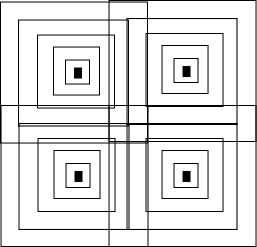
\includegraphics[width=30em \textwidth]{./manhattan_effect.png}
\caption{Manhattan effect.}
\end{figure}
\section{Implementation of Fawcett's \cite{fawcett08} idea}
\label{sec-4}



The programming language chosen is C++ making use of Standard Template
Library (STL).  This is a command line programme, which needs to
parameters passed to it, the path to the file containing the training
data and the path to the file containing the test data.

Fawcett \cite{fawcett08} used data sets from from UCI Machine Learning
Repository \href{http://archive.ics.uci.edu/ml/index.html}{http://archive.ics.uci.edu/ml/index.html}.  For this
implementation the Iris data set is used.

To be able to use any data sets for this programme, they must be
transformed into a format the programme can use, and predicate values
must be transformed into integer form, so they can be used as
addresses for the array which represents the grid.  A value of 0.23
can not be used as a address in a computer array.  Also string values
for classes can not be used in this implementation as only integer
values are supported.  Also the data needs to be split into training
and test data. 

To do this transformation a python script was created. The source is
shown below to illustrate what has to be done to make data usable by
this programme. 

\lstset{language=Python}
\begin{lstlisting}
#all data is gained from the file 'iris.data' found in the data folder,
#which the script is also run from.

#'iris.data' is in a csv format so can be processed by the csv module
import csv

#A dictionary to use to transform the class names into integers
name = {'Iris-setosa':1, 'Iris-versicolor':2, 'Iris-virginica':3 }

#create the test data outputing to 'iris_test.data'
with open('iris_test.data', 'w') as data:
    abareader = csv.reader(open('iris.data'))
    #interate through a list comprising of every 4th item in the data list
    for row in list(abareader)[::4]:
        #interate over the first 4 items in the row
        for x in row[0:4]:
            #transform the float values into integer values
            #by multiplying by 10 and discarding anything after decimal point
            print >>data, "%2d"%(int(round(float(x)*10))),
        #make the class name a integer
        print >>data, "%d" % (int(name[row[4]]))


#create the training data outputing to iris_train.data
with open('iris_train.data', 'w') as data:
    abareader = csv.reader(open('iris.data'))
    tmp = list(abareader)#the entire list
    tmp2 = tmp[::4]#represents the testing data
    #interate over a diff between the 2 lists, tmp and tmp2
    for row in [i for i in tmp+tmp2 if i not in tmp or i not in tmp2]:
        for x in row[0:4]:
            print >>data, "%2d"%(int(round(float(x)*10))),
        print >>data, "%d" % (int(name[row[4]]))
\end{lstlisting}
\section{Results}
\label{sec-5}


\begin{lstlisting}
begin
before init graph
graph size = 6552000
graph size = 6552000
after init graph

loading training data from data/iris_train.data

number of classes: 3
classes: 1 2 3 
Number of dimensions: 4

running CA until convergence

0% done
been going for 0 steps
0% done
been going for 5 steps
1% done
been going for 10 steps
4% done
been going for 15 steps
10% done
been going for 20 steps
18% done
been going for 25 steps
27% done
been going for 30 steps
38% done
been going for 35 steps
48% done
been going for 40 steps
58% done
been going for 45 steps
67% done
been going for 50 steps
75% done
been going for 55 steps
82% done
been going for 60 steps
88% done
been going for 65 steps
92% done
been going for 70 steps
96% done
been going for 75 steps
98% done
been going for 80 steps
99% done
been going for 85 steps
100% done
finished 100% done

loading test data from data/iris_test.data
running tests
results of test are:
passed 38 / 38
\end{lstlisting}
  \href{http://archive.ics.uci.edu/ml/index.html}{http://archive.ics.uci.edu/ml/index.html}
\section{Conclusions}
\label{sec-6}

  
\section{Future work}
\label{sec-7}


\begin{itemize}
\item Extend the cellular automata to find the best predicates and divide
   the data into test and train and use this data to create and test
   itself as a classifier.
\end{itemize}

\bibliographystyle{plain}
\bibliography{bibliography}

\end{document}
